\chapter{Facial Recognition}\label{ch:face-rec}
Facial recognition is a task of verifying or identifying a person from digital image/video.

As I mentioned in the definition, there are two main subtasks~\cite{FaceRec}:
\begin{enumerate}
    \item \textbf{Verification} deals with verifying whether the person in the image is who he claims he is.
    Typical modern use case of verification is smartphone unlocking with face.
    An example of such system is Face ID developed by Apple Inc.

    \item \textbf{Identification} is a task of matching a person to an identity.
    To formulate it in another way, the goal of identification is to give us an answer to the question of who the person
    in the image is.
\end{enumerate}

\section{Pipeline}\label{sec:pipeline}

Facial recognition pipeline\footnote{A chain of processing elements, arranged so that the output of each element is the
input of the next.} usually has the following four steps:
\begin{enumerate}
    \item The first on is \textbf{face detection} and it deals with determination of face location within the image.
    The output of the algorithm is usually face coordinates and facial landmarks.
    Landmarks are a set of coordinates marking important points of the face (eyebrows, nose, mouth, \ldots).
    The knowledge of these points is a necessity for the following step.
    \item \textbf{Face alignment} is a task of changing the face position in such a way that it resembles the position
    of faces on which the feature extraction model was trained.
    In most of the instances this step improves the accuracy.
    \item \textbf{Feature extraction} is a process of computing a feature vector\footnote{A feature vector is a vector
    that contains information describing an object's important characteristics.} of the face.
    Architecture of models used for feature extraction is described in section~\ref{sec:mod-methods}.
    \item \textbf{Feature matching} uses feature vector from the previous task to identify the person in the image.
    The algorithm uses a database of pre-computed feature vectors and compares them to the newly extracted one.
    The identity associated with the feature vector which has the smallest distance from the extracted one is
    considered to be the identity of the person in the image.
\end{enumerate}

\section{Overview of Modern Methods}\label{sec:mod-methods}
In this section I am about to provide an overview of modern methods/models used for facial recognition.
Models based on CNN architecture~\ref{ch:cnn} achieve state-of-the-art results which is the reason why CNNs dominate the
field of facial recognition and the field of computer vision as a whole now.

Innovations made in the field of computer vision are usually applicable to the subfield of facial recognition as well.
This is manifested in usage of the same model architectures in general image classification as well as in facial
recognition.
However there is a lot of innovation going on in the design of loss functions which work specifically well when used for
model training\footnote{Machine learning task of learning a function that maps an input to an output based on example
input-output pairs.} in facial recognition tasks.
This is the reason why this section is divided in two parts: \textit{models}~\ref{subsec:models} and
\textit{loss functions}~\ref{subsec:loss-functions}.

\subsection{Models}\label{subsec:models}

\subsubsection{DeepFace}\label{subsec:deepface}
DeepFace~\cite{DeepFace} is a system developed by FaceBook Inc. in 2014.

The research is notable for its use of advanced alignment technique which consists of three steps:

\begin{enumerate}
    \item The first step is \textbf{2D Alignment} and it begins with detection of 6 fiducial points/landmarks.
    These points and the reference position of points are then used to find a transformation.
    This transformation then generates 2D aligned and cropped image.
    \item The second step is \textbf{3D Alignment}.
    In this step the image is warped onto a generic 3D shape model.
    This is achieved by localization of 67 fiducial points in the image and then fitting an affine
    camera\footnote{linear mathematical model to approximate the perspective projection followed by an ideal
    pinhole camera.} \textit{P} using the generalized least squares solution and the reference position $x_{3d}$ of
    points on the 3D shape model.
    \item \textbf{Frontalization} is the final step and it is achieved by a piece-wise affine transformation T from
    $x_{2d}$ source to $\tilde{x_{3d}}$ target.
    The target $\tilde{x_{3d}}$ is a list of positions of reference fiducial points from previous step enriched with
    residuals \textit{r}.
    These residuals were added to the reference positions $\tilde{x_{3d}}$ to account for non-rigid deformations which
    are not modeled by the affine camera \textit{P}.
    Without these residuals, all faces would be warped into the same shape losing important discriminative factors.
\end{enumerate}

\begin{figure}[H]
    \centering
    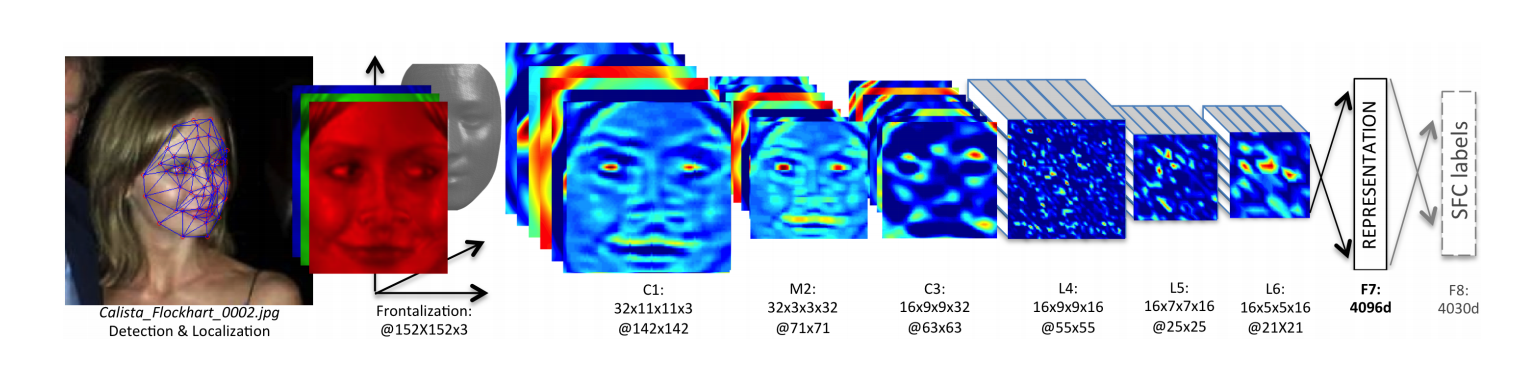
\includegraphics[width=\columnwidth]{images/face-recognition/deepface.png}
    \caption{Outline of DeepFace architecture~\cite{DeepFace}}
    \label{fig:deepface}
\end{figure}



\subsubsection{FaceNet}\label{subsec:facenet}
\subsubsection{ResNet}\label{subsec:resnet}
\subsubsection{InceptionNet}\label{subsec:inceptionnet}
\subsubsection{DenseNet}\label{subsec:densenet}

\subsection{Loss Functions}\label{subsec:loss-functions}